\documentclass[12pt,a4paper]{article}
\usepackage[margin=1in]{geometry}
\usepackage[T1]{fontenc}
\usepackage{lmodern}
\usepackage{microtype}
\usepackage{amsmath,amssymb}
\usepackage{booktabs,array,tabularx}
\usepackage{graphicx}
\usepackage{xcolor}
\usepackage{tikz}
\usetikzlibrary{arrows.meta,positioning,fit}
\usepackage{caption}
\usepackage{titlesec}
\titlespacing*{\section}{0pt}{5pt}{2pt}
\usepackage{hyperref}
\usepackage{xurl}
\hypersetup{colorlinks=true,linkcolor=black,urlcolor=blue!55!black}
\urlstyle{tt}
\setlength{\parindent}{0pt}
\setlength{\parskip}{2pt}
\setlength{\emergencystretch}{3em}
\setlength{\abovecaptionskip}{4pt}
\setlength{\belowcaptionskip}{2pt}
\captionsetup{font=small,labelfont=bf}
\definecolor{naf}{HTML}{F4A261}
\definecolor{cond}{HTML}{8ECAE6}
\definecolor{wav}{HTML}{90BE6D}
\definecolor{ink}{HTML}{23313D}
\color{ink}
\newcommand{\codepath}[1]{\begingroup\small\ttfamily\raggedright\path{#1}\par\endgroup}

\begin{document}

\begin{center}
{\large\bfseries Noise-Conditioned Wavelet NAFNet for Blind Low-Light sRGB Denoising\par}
\vspace{0.3em}
{\normalsize Team Voxel \quad---\quad Mora SP Cup 2026, Preliminary Round}\par
\end{center}
\vspace{-0.3em}

\section{Problem and scoring objective}
The task is blind denoising of $992\times992$ 8-bit sRGB low-light photographs. Corruption strength varies per image and no noise-level metadata is available at inference. The official score is computed per image and averaged:
\begin{equation}
\mathrm{composite}=0.6\,\mathrm{clip}\!\left(\tfrac{\Delta\mathrm{PSNR}}{15},0,1\right)+0.4\,\max(\Delta\mathrm{SSIM},0),
\end{equation}
each delta measured against the noisy input. The $0.6/15=0.04$ gain per dB makes the metric PSNR-led while SSIM rewards structure preservation. Because the clip and the max are applied \emph{before} averaging, per-image robustness matters more than mean performance. The model therefore predicts a residual at the original exposure and performs no gamma correction, tone mapping or global brightness adjustment.

\section{Dataset observations}
The 460 public noisy/clean pairs were characterised before any model was built. Residual variance is heteroscedastic and follows a Poisson--Gaussian law $\operatorname{var}(I)=aI+b$, with normalised per-channel coefficients
\[
a=(0.017095,\,0.016532,\,0.019045),\qquad b=(0.006362,\,0.005684,\,0.005492).
\]
Three further observations drive the design. The read-noise floor $b$ dominates dark regions, so corruption is strongest exactly where signal is weakest. Severity forms a \emph{continuum} rather than discrete levels, which rules out a classifier over noise levels. And the residual is heavy-tailed with sparse impulses --- 492 persistent hot pixels plus scattered defects --- which a Gaussian model cannot represent. Together these motivate \emph{spatial, content-dependent} conditioning rather than a single global noise scalar.

\section{Classical signal processing}
Three components operate directly on the noisy observation and carry \textbf{no learned parameters}. They supply the network with physical knowledge it would otherwise have to infer from data.

\textbf{1. Analytical noise map.} Evaluating $\sqrt{aI+b}$ with the fitted coefficients yields a per-pixel, per-channel standard-deviation estimate. This is the measured sensor model applied pointwise: the network is told how much corruption to expect at each intensity, instead of estimating it from a $256\times256$ patch where the estimate would be unreliable in dark or flat regions.

\textbf{2. Exact $3\times3$ median via a sorting network.} Impulse defects are not describable by a variance model, so they are detected separately. Nine replicate-padded neighbour tensors are sorted elementwise by a 36-comparison min/max bubble network; element four is the exact median. The channel-max absolute deviation from that median, scaled and clipped, becomes a one-channel impulse-confidence map. A sorting network is used rather than a library median because it is differentiable, backend-portable and exact --- no histogram approximation.

\textbf{3. Four-level orthonormal Haar pyramid.} The LL band is recursively decomposed; at each scale the RGB LH, HL and HH details form nine channels at $H/2,\dots,H/16$. This is a fixed filter bank, so the detail bands are a deterministic function of the input. Wavelet details expose high-frequency corruption at multiple scales \emph{without} altering the RGB tensor the backbone consumes --- the restoration path still sees the original observation.

Feeding these as \emph{conditioning} rather than as extra input channels is deliberate: it leaves the pretrained backbone's input distribution untouched, so the wrapper can be initialised to an exact identity (Section~5).

\section{Architecture}
\textbf{Backbone.} NAFNet (width 32) with encoder depths $[2,2,4,8]$, 12 middle blocks, decoder depths $[2,2,2,2]$ and channel widths $32,64,128,256,512$. Each NAFBlock uses LayerNorm, pointwise expansion, depthwise $3\times3$ convolution, SimpleGate, simplified channel attention and two learned residual scales. PixelShuffle performs decoder upsampling; the network predicts a residual added to the reflect-padded input.

\begin{figure}[h]
\centering
\resizebox{0.97\textwidth}{!}{%
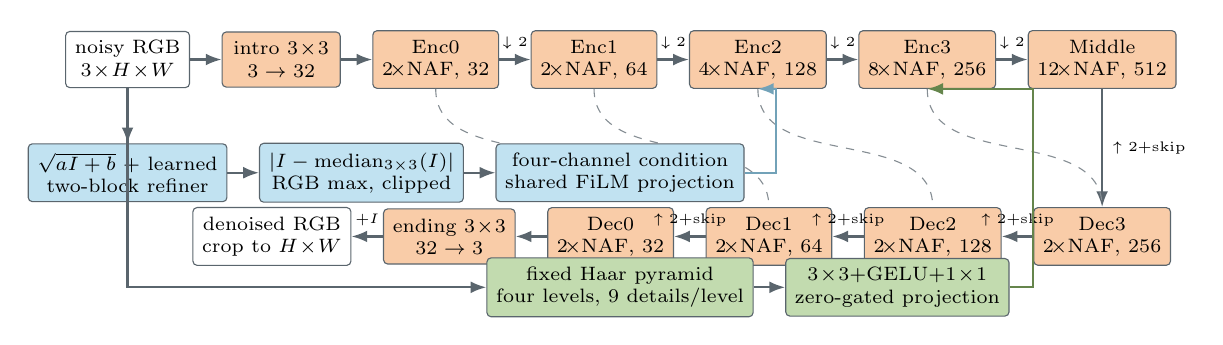
\begin{tikzpicture}[
  node distance=3.5mm and 4mm,
  box/.style={draw=ink!75,rounded corners=1.5pt,minimum height=7mm,minimum width=15mm,align=center,font=\scriptsize},
  core/.style={box,fill=naf!55}, cb/.style={box,fill=cond!55}, wb/.style={box,fill=wav!55},
  arr/.style={-{Latex[length=2mm]},thick,draw=ink!75}]
\node[box] (in) {noisy RGB\\$3\!\times\!H\!\times\!W$};
\node[core,right=of in] (intro) {intro $3\!\times\!3$\\$3\to32$};
\node[core,right=of intro] (e0) {Enc0\\$2\!\times$NAF, 32};
\node[core,right=of e0] (e1) {Enc1\\$2\!\times$NAF, 64};
\node[core,right=of e1] (e2) {Enc2\\$4\!\times$NAF, 128};
\node[core,right=of e2] (e3) {Enc3\\$8\!\times$NAF, 256};
\node[core,right=of e3] (mid) {Middle\\$12\!\times$NAF, 512};
\draw[arr] (in)--(intro); \draw[arr] (intro)--(e0);
\draw[arr] (e0)--node[above,font=\tiny]{$\downarrow2$}(e1);
\draw[arr] (e1)--node[above,font=\tiny]{$\downarrow2$}(e2);
\draw[arr] (e2)--node[above,font=\tiny]{$\downarrow2$}(e3);
\draw[arr] (e3)--node[above,font=\tiny]{$\downarrow2$}(mid);
\node[core,below=15mm of mid] (d3) {Dec3\\$2\!\times$NAF, 256};
\node[core,left=of d3] (d2) {Dec2\\$2\!\times$NAF, 128};
\node[core,left=of d2] (d1) {Dec1\\$2\!\times$NAF, 64};
\node[core,left=of d1] (d0) {Dec0\\$2\!\times$NAF, 32};
\node[core,left=of d0] (end) {ending $3\!\times\!3$\\$32\to3$};
\node[box,left=of end] (out) {denoised RGB\\crop to $H\!\times\!W$};
\draw[arr] (mid)--node[right,font=\tiny]{$\uparrow2+$skip}(d3);
\draw[arr] (d3)--node[above,font=\tiny]{$\uparrow2+$skip}(d2);
\draw[arr] (d2)--node[above,font=\tiny]{$\uparrow2+$skip}(d1);
\draw[arr] (d1)--node[above,font=\tiny]{$\uparrow2+$skip}(d0);
\draw[arr] (d0)--(end); \draw[arr] (end)--node[above,font=\tiny]{$+I$}(out);
\draw[dashed,draw=ink!55] (e0.south) to[out=-90,in=90] (d0.north);
\draw[dashed,draw=ink!55] (e1.south) to[out=-90,in=90] (d1.north);
\draw[dashed,draw=ink!55] (e2.south) to[out=-90,in=90] (d2.north);
\draw[dashed,draw=ink!55] (e3.south) to[out=-90,in=90] (d3.north);
\node[cb,below=7mm of in] (ana) {$\sqrt{aI+b}$ + learned\\two-block refiner};
\node[cb,right=of ana] (imp) {$|I-\mathrm{median}_{3\times3}(I)|$\\RGB max, clipped};
\node[cb,right=of imp] (film) {four-channel condition\\shared FiLM projection};
\draw[arr] (in)--(ana); \draw[arr] (ana)--(imp); \draw[arr] (imp)--(film);
\draw[arr,draw=cond!80!black] (film.east) -- ++(4mm,0) |- (e2.south);
\node[wb,below=7mm of film] (haar) {fixed Haar pyramid\\four levels, 9 details/level};
\node[wb,right=of haar] (adapt) {$3\!\times\!3+$GELU$+1\!\times\!1$\\zero-gated projection};
\draw[arr] (in.south) |- (haar.west); \draw[arr] (haar)--(adapt);
\draw[arr,draw=wav!70!black] (adapt.east) -- ++(3mm,0) |- (e3.south);
\end{tikzpicture}}
\caption{NCW-NAFNet. The NAFNet core is orange, noise conditioning blue, fixed-Haar detail injection green. Dashed lines are encoder--decoder skips.}
\end{figure}

\textbf{Noise conditioning.} The analytical branch computes $\sqrt{aI+b}$; a 16-channel, two-NAFBlock refiner predicts a $\tanh$-bounded correction of at most $\pm0.1$, letting the model adapt the global sensor model to individual images. Concatenating the three sigma channels with the impulse channel gives a four-channel field $C$. At every encoder stage and at the middle block a shared $3\times3$ projection with two $1\times1$ heads generates FiLM parameters:
\[
F'=(1+g_\gamma\tanh\gamma(C))\odot F+g_\beta\beta(C).
\]
Conditioning is applied \emph{before} the encoder output is stored as a skip, so the decoder also receives conditioned features.

\textbf{Wavelet conditioning.} At each scale a $3\times3\to\mathrm{GELU}\to1\times1$ adapter projects the nine Haar detail channels to the matching feature width and adds them after downsampling, through a zero-initialised scalar gate. Level $\ell$ injects at exactly the resolution produced by downsample $\ell$, so no resampling occurs.

The model has 29{,}664{,}484 parameters: 29{,}159{,}715 in the backbone and 504{,}769 in the added modules --- a 1.7\,\% parameter increase.

\section{Identity safety}
Every added path is scaled by a scalar gate initialised to zero, so before training the wrapper output is \emph{numerically identical} to the backbone. This is a design guarantee, not an approximation: the preflight check measured a maximum absolute difference of exactly $0.0$, and the property is asserted by a unit test in \codepath{scripts/tests/test_model.py}. It means conditioning can only be adopted where it earns its place, and an untrained adapter can never destroy the restoration capability of the backbone.

Two repairs were needed on the DirectML backend: AdamW's in-place \texttt{lerp\_} was replaced by an equivalent \texttt{addcmul\_}/\texttt{addcdiv\_} update, and whole-image validation was replaced by CPU-staged tiling. The official evaluator still scores complete $992\times992$ predictions.

\section{Training protocol}
Training ran in float32 on DirectML with batch size 1 and random $256\times256$ patches. Each sample was a real noisy/clean pair with probability 0.70; otherwise a clean patch was corrupted by a generalised synthesiser fitted to the measured statistics, with randomised $a$/$b$ scaling, heavy-tail mixing and sparse defects. The objective was $L=0.90L_{\mathrm{PSNR}}+0.10L_{\mathrm{SSIM}}$ with gradient norm clipped at 1.0, $\beta=(0.9,0.9)$ and weight decay $10^{-3}$.

\begin{table}[h]
\centering\small
\begin{tabularx}{\textwidth}{@{}>{\raggedright\arraybackslash}p{0.17\textwidth}>{\raggedright\arraybackslash}p{0.15\textwidth}>{\raggedright\arraybackslash}X>{\raggedright\arraybackslash}p{0.24\textwidth}@{}}
\toprule
Phase & Interval & Trainable parameters & Backbone / adapter LR \\
\midrule
A: adapter activation & steps 0--999 & NCW additions only & $0\,/\,3.0\times10^{-4}$ \\
B: targeted tuning & steps 1000--3424 & middle, decoder, output + NCW & $3.0\times10^{-5}\,/\,1.5\times10^{-4}$ \\
C: low-LR refinement & steps 3425--4122 & full model & cosine from $1.2\times10^{-5}\,/\,7.0\times10^{-5}$ \\
\bottomrule
\end{tabularx}
\caption{Three phases. Phase C decayed to $1.8\times10^{-6}/1.05\times10^{-5}$ at the optimizer cutoff. Freezing the backbone during phase A lets the gates open before any pretrained weight moves.}
\end{table}

Optimisation stopped at 52 minutes to reserve time for full validation and checkpoint selection, completing 4{,}122 steps and five validation epochs in 58.3 minutes.

\section{Validation methodology and results}
The 460 public pairs are split \emph{deterministically and without RNG}: ids are ordered by blind noise estimate and every tenth is held out starting at index five, giving 414 training and 46 validation images spanning the full severity continuum ($\hat\sigma$ 7.57--40.66) rather than whichever end a random draw favoured. The split is regenerated on demand, so no stored state can drift. Image IDs 461--480 were excluded from all fitting, checkpoint selection and metric computation.

Every prediction is clipped, quantised round-half-up as $\lfloor255x+0.5\rfloor$, written as PNG and scored by the \emph{unmodified} \texttt{evaluation/evaluate.py}. The reported figures therefore include the exact 8-bit quantisation used for the submitted images.

\begin{table}[h]
\centering\small
\begin{tabular}{@{}r r c r r r@{}}
\toprule
Epoch & Step & Phase & PSNR (dB) & SSIM & Composite \\
\midrule
1 & 1000 & A & 31.3039 & 0.919125 & 0.634218 \\
2 & 2000 & B & 31.2968 & 0.918920 & 0.634052 \\
3 & 3000 & B & 31.3027 & 0.919209 & 0.634348 \\
4 & 4000 & C & 31.3075 & 0.919298 & 0.634611 \\
\textbf{5} & \textbf{4122} & \textbf{C} & \textbf{31.3046} & \textbf{0.919337} & \textbf{0.634625} \\
\midrule
\multicolumn{3}{l}{Provided starter baseline} & --- & --- & $\approx0.26$ \\
\bottomrule
\end{tabular}
\caption{Validation trajectory over all 46 held-out images. Epoch 4 maximises PSNR; epoch 5 maximises the official composite and is the submitted checkpoint.}
\end{table}

The selected checkpoint achieves \textbf{31.3046\,dB PSNR}, \textbf{0.919337 SSIM} and \textbf{0.63462481 composite} --- roughly $2.4\times$ the provided baseline's composite of $\approx0.26$, and a mean improvement of $+11.49$\,dB PSNR and $+0.4634$ SSIM over the noisy inputs. Checkpoint selection used the official composite rather than PSNR: step 4122 trades $0.0029$\,dB for a $3.9\times10^{-5}$ SSIM gain, which the $0.6/0.4$ weighting rewards. Composite varies by only $0.00057$ across the five epochs, indicating a stable, converged run rather than a lucky draw.

\textbf{Released checkpoint.} Weights ship in float16 (57\,MB rather than 178\,MB) and are upcast to float32 at load. Re-scored on CPU, the released file gives \textbf{31.3054\,dB}, \textbf{0.919342}, \textbf{0.63464547} --- $+2.0\times10^{-5}$ composite against the float32 original, with outputs differing by at most one 8-bit level on under 3\,\% of pixels.

\begin{figure}[h]
\centering
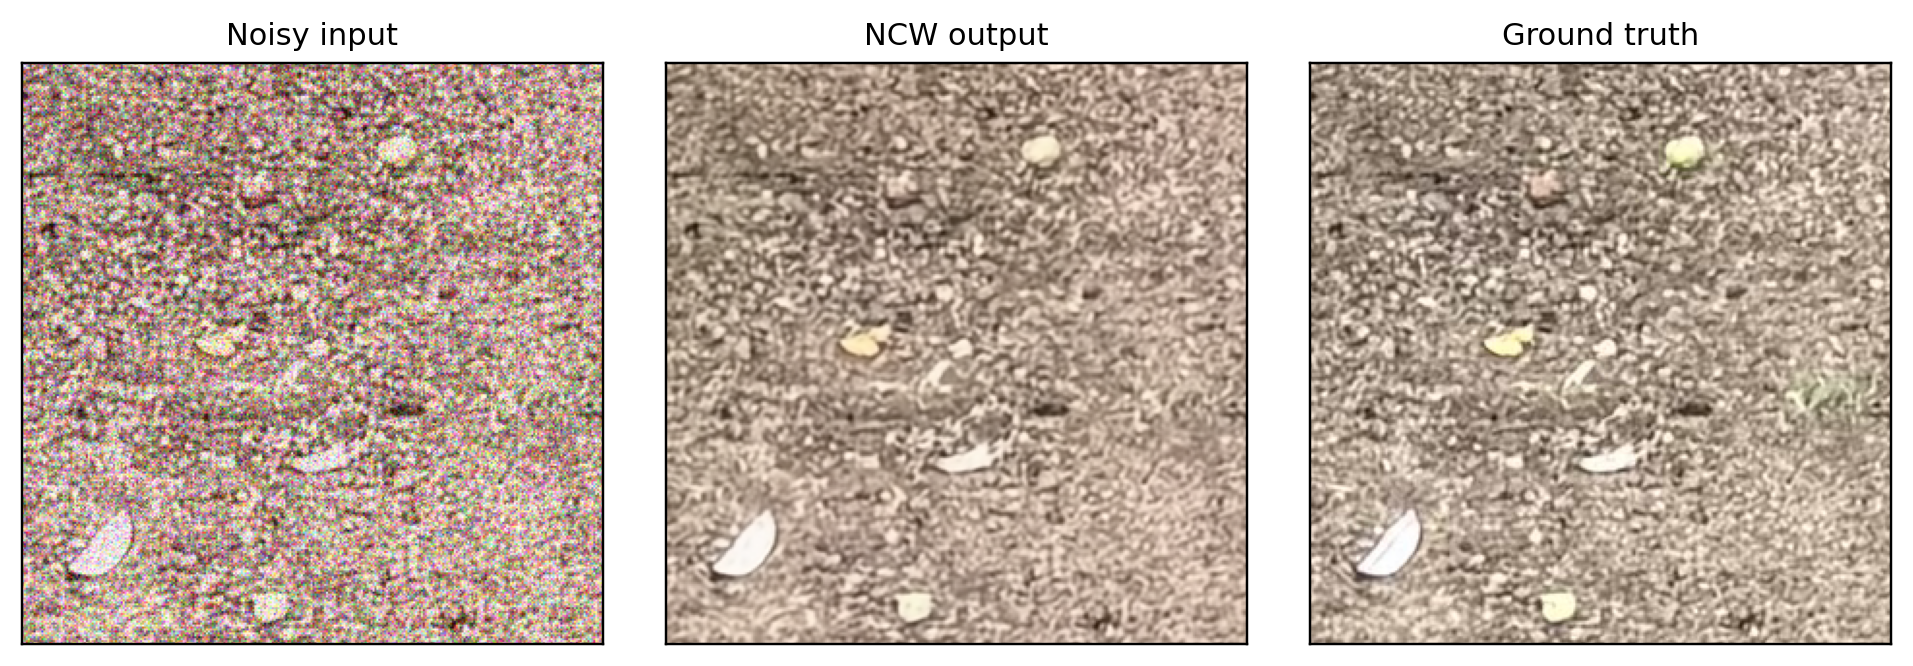
\includegraphics[width=0.60\textwidth]{figs/qualitative_183.png}
\vspace{-2pt}
\caption{Centre crops for validation image 183, the most severe held-out image by blind noise estimate ($\hat\sigma=40.66$ in 8-bit units). Strong noise is removed while the original exposure is retained.}
\end{figure}

\textbf{Alternatives considered.} Feeding the conditioning maps as additional input channels was rejected because it changes the backbone's input distribution and forecloses identity initialisation. Predicting a global noise scalar was rejected because measured severity is a continuum with strong spatial variation. Gamma correction and tone mapping were rejected outright: the metric compares against ground truth at the original exposure, so any brightness change is a direct PSNR loss.

\section{Reproducibility}
Inference is deterministic, CPU-capable and offline, using 256-pixel tiles with a 64-pixel discarded context halo and a raised-cosine blend over a 64-pixel overlap. The checkpoint embeds its own resolved configuration and metrics, so the model is rebuilt from the file itself and loaded with \texttt{strict=True} over all 766 tensors.

\codepath{python scripts/denoise.py --noise_dir <in> --denoised_dir <out>}
\codepath{python scripts/validate.py}

Submitted checkpoint \codepath{scripts/weights/ncw_1h_best_composite_fp16.pth}
SHA-256 \codepath{be1515a1afe066bbd445b6a5b73f04d0141d3ed08e22eaa4cb9fd145df86155b}

\vspace{0.3em}
{\footnotesize\textbf{Backbone reference:} S. Chen et al., ``Simple Baselines for Image Restoration,'' ECCV 2022 (MIT licence, retained in \texttt{scripts/licenses/}). All metrics in this report are produced by the organizers' unmodified evaluator; no value is extrapolated from training loss.}

\end{document}
